%
%                  Politecnico di Milano
%
%         Student: Caravano Andrea
%            A.Y.: 2023/2024
%
%   Last modified: 10/09/2024
%
%     Description: Wireless Internet/Wireless Networks project: Wi-Fi encrypted traffic classification
%

\documentclass[a4paper,11pt]{article} % tipo di documento
\usepackage[T1]{fontenc} % codifica dei font
\usepackage[utf8]{inputenc} % lettere accentate da tastiera
\usepackage[english,italian]{babel} % lingua del documento
\usepackage{lipsum} % genera testo fittizio
\usepackage{url} % per scrivere gli indirizzi Internet e/o di riferimento nella pagina

\usepackage[hidelinks]{hyperref} % per modificare il comportamento dei collegamenti ipertestuali (+ leva colore attorno)

\usepackage[margin=0.7in]{geometry} % margine di pagina

\usepackage{graphicx} % per inserire immagini

\usepackage[outputdir=../auxil]{minted} % per colorazione automatica del codice (installare pygments da Homebrew)
% \usepackage{pythonhighlight} % per Python

\setminted{ % si può impostare il linguaggio specifico con \setminted[JSON] ad esempio
    linenos=true,
    breaklines=true,
    encoding=utf8,
    fontsize=\normalsize,
    frame=lines
}

\usepackage{fancyhdr}
\usepackage{textcomp} % per gestione intestazione e piè di pagina

\hypersetup{ % metadati di titolo e autore nel PDF
    pdftitle={Wireless Internet project - A.Y. 2023/24},
    pdfauthor={Andrea Caravano}
}

\setlength{\parindent}{0pt} % rimuove l'indentazione del testo

\begin{document}
    \pagestyle{fancy}
    \fancyhead{}\fancyfoot{}
    \fancyhead[L]{\textbf{Wireless Internet project}}
    \fancyhead[R]{Andrea Caravano}
    \fancyfoot[C]{\thepage}

    \title{\textbf{Wireless Internet project}\\Wi-Fi encrypted traffic classification}
    \author{Andrea Caravano}
    \date{Academic Year 2023--24}
    \maketitle


    \section{Project requirements}\label{sec:project-requirements}

    \subsection{Specifications}\label{subsec:specifications}

    Implement a machine-learning classifier able to distinguish what kind of activity a user is performing with his/her smartphone/laptop by sniffing traffic in monitor mode.

    The system should perform the following operations:

    \begin{itemize}
        \item Sniff traffic in monitor mode from a known MAC address
        \item Extract statistical features from the traffic every W seconds.
        The following traffic features can be extracted: number of packets up/down, average and variance of the packet size, average and variance of the inter-arrival packet times etc.
        \item Use a pre-trained machine-learning classifier of your choice to recognize the user activity among at least the following: idle, web browsing, YouTube streaming.
        \item Report the accuracy of the approach through a confusion matrix
    \end{itemize}


    \section{Snippets}\label{sec:snippets}

    \subsection{Traffic types}\label{subsec:traffic-types}

    The final dataset is prepared alongside the target address (the one on which statistical indexes are extracted) and traffic types.

    \begin{minted}{Python}
target_addr = '8a:c4:06:ee:1d:83' # target address on which we are applying the ML algorithm

dataset = [] # final datasets
traffic_types = ['youtube', 'speedtest', 'web', 'idle']
    \end{minted}

    Chosen traffic types are:

    \begin{itemize}
        \item Idle: no relevant user activity

        Modern smartphones are still expected to exchange push/pull notifications frames and, eventually, reply to broadcast inquiries, if any
        \item Web browsing: news sources, emails and search engine queries
        \item YouTube video streaming: buffering is strongly used in the mobile context, so the packet flow is expected to be quite similar to the web browsing one
        \item Speedtest: several Ookla's Speedtests, the packet flow traits are expected to be quite unique
    \end{itemize}

    \subsection{Data extraction}\label{subsec:data-extraction}

    Valid packets are then kept and their fields stored to be finally gathered for statistical analysis.

    \begin{minted}{Python}
  # Processing of packets
  for frame in cap:
    count += 1 # overall count
    success = False # malformed packets

    try:
      layers = frame.layers # pointer to layers
      timestamp = frame.sniff_timestamp # TS in ms
      sa = layers[2].sa # 802.11 frame: Source address
      da = layers[2].da # 802.11 frame: Destination address
      length = int(frame.length) # frame length
      success = True # packet is non malformed
    except:
      failed += 1 # processing failed: counting the packet as malformed
      success = False
    \end{minted}

    As per project specifications, in both directions, the following statistical figures are used to form training and testing sets:

    \begin{itemize}
        \item Number of packets
        \item Average and variance of packet size
        \item Average and variance of inter-arrival packet times
    \end{itemize}

    The approach followed is the same applied for localization fingerprinting, from which the resulting outcomes are observed.

    \subsection{Classification}\label{subsec:classification}

    \begin{minted}{Python}
X_train, X_test, y_train, y_test = train_test_split(X_norm, Y, test_size=0.5) # 50% will be used for the training set, the rest for the testing set

# K-NeirestNeighbor (up to 4)
# as seen for localization fingerprinting
ACCURACY = []
for k in range(1,5):
  knn = KNeighborsClassifier(n_neighbors=k, weights='distance')
  knn.fit(X_train, y_train)
  knn_predict = knn.predict(X_test)
  accuracy = accuracy_score(y_test, knn_predict)
  ACCURACY.append(accuracy)

# we finally plot the confusion matrix
bestk = np.argmax(ACCURACY)+1
knn = KNeighborsClassifier(n_neighbors=bestk, weights='distance')
knn.fit(X_train, y_train)
knn_predict = knn.predict(X_test)
fig, ax = plt.subplots(figsize=(15, 15));
ConfusionMatrixDisplay.from_predictions(knn_predict, y_test, ax=ax, normalize='true');
    \end{minted}


    \section{Outcome}\label{sec:outcome}

    \subsection{Confusion Matrix}\label{subsec:confusion-matrix}

    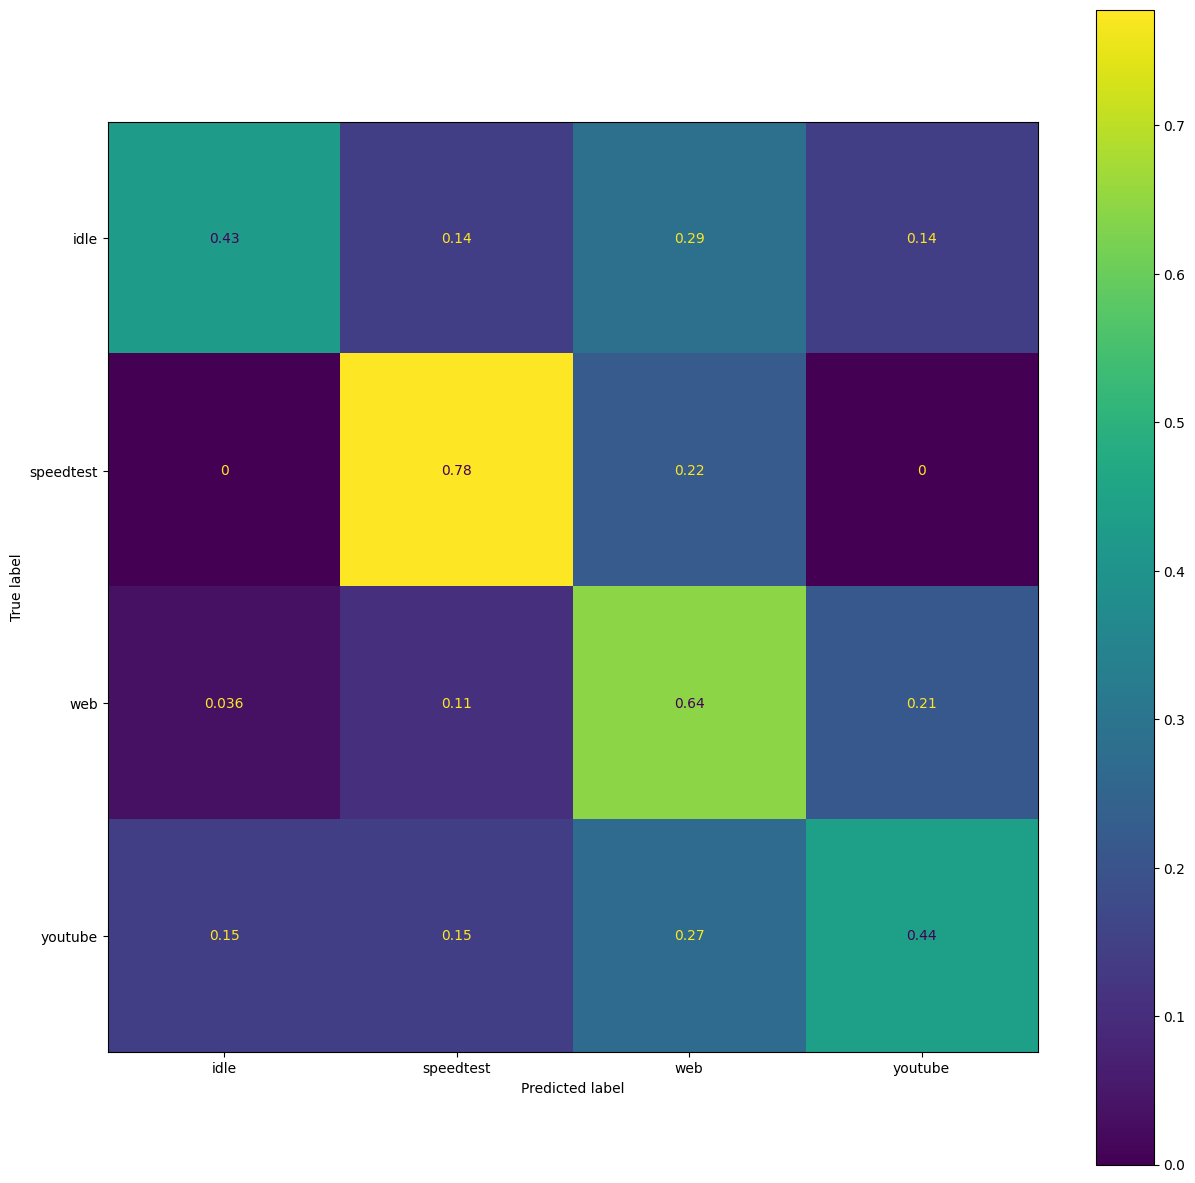
\includegraphics[height=17cm]{../res/confusion-matrix}

    \subsection{Comment}\label{subsec:comment}

    The speedtest traffic classifier stands out as the most accurate, as anticipated.

    \medskip

    Web traffic is the next one: its traffic figures are influenced by the adoption of buffering in the YouTube streaming case, resulting in mostly uniform characteristics.

    \medskip

    YouTube streaming and idle traffic models have the highest imprecisions: this is also expected, since buffering hides the few bursts of traffic flowing, resulting in less distinguishable traffic traits.
\end{document}
